\section{Supplementary Historical Loopback Evidence}

This appendix contains the five additional plots from the historical 21-run cohort. It does not add new measurements or pool the old loopback results with the revised veth experiment. Historical rate-sweep points average three run-level statistics and error bars show minimum--maximum, not confidence intervals.

\subsection{Application payload goodput}

Payload bytes in successful completions inside the 60 s window were summed, converted to bits and divided by the window duration. Metadata, protocol headers and acknowledgement responses are excluded. The dashed line denotes configured payload offered across all classes.

\begin{figure}[H]
\centering
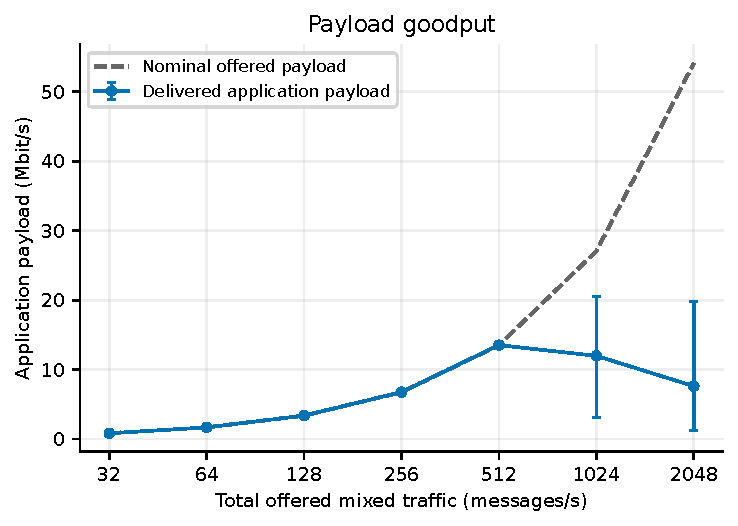
\includegraphics[width=0.88\linewidth]{figures/historical_appendix_goodput.pdf}
\caption{Historical loopback application payload goodput. Points average three runs; bars show minimum--maximum. The horizontal rate includes all four classes.}
\label{fig:e1r-historical-appendix-goodput}
\end{figure}


Goodput averaged 13.53 Mbit/s at nominal 512 messages/s and 7.62 Mbit/s at nominal 2,048 messages/s, despite 54.1184 Mbit/s of configured payload offered at the latter load. Useful payload and completed request count answer different questions when message sizes and the delivered class mix differ.

\subsection{Admission loss under overload}

Each run's FIFO-drop count was divided by its generated measurement-cohort count; the plot averages those three fractions. This differs from pooling all messages before computing a fraction, although the reported rounded values are close.

\begin{figure}[H]
\centering
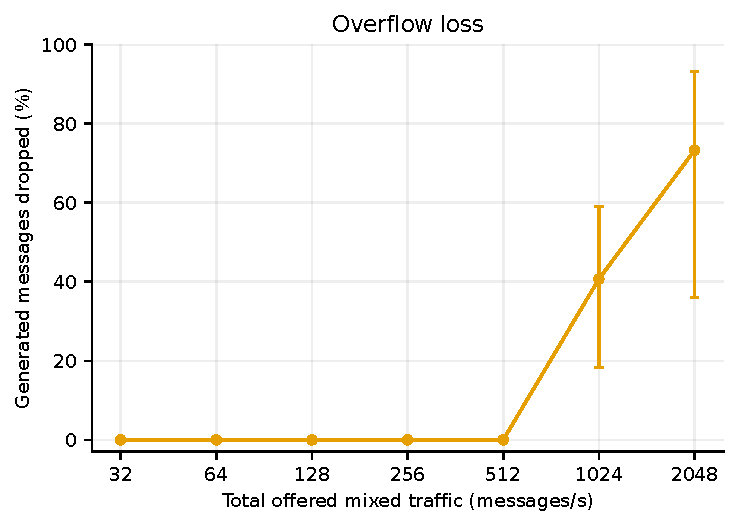
\includegraphics[width=0.88\linewidth]{figures/historical_appendix_drops.pdf}
\caption{Historical FIFO admission-drop percentage versus total offered mixed traffic. Points average three run fractions; bars show minimum--maximum.}
\label{fig:e1r-historical-appendix-drops}
\end{figure}


Mean per-run FIFO-drop percentages were 40.68\% at nominal 1,024 messages/s and 73.27\% at nominal 2,048/s. These are application admission losses. The rejected messages were never sent as HTTP requests.

\subsection{Queue evolution in selected repetitions}

The piecewise-constant waiting-queue state was sampled every 100 ms during repeat 1 at nominal 512, 1,024 and 2,048 messages/s. The same repeat index is selected at every load; this is not a best-run selection. Repeat indices do not indicate chronological run order.

\begin{figure}[H]
\centering
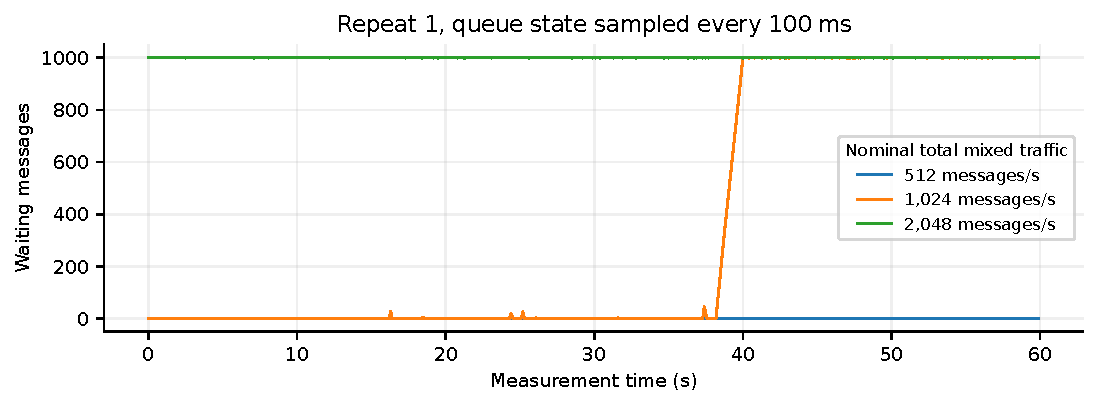
\includegraphics[width=0.88\linewidth]{figures/historical_appendix_queue_trace.pdf}
\caption{Historical waiting-queue traces for repeat 1 of the three highest nominal total traffic rates. Legend values are messages/s across all four classes.}
\label{fig:e1r-historical-appendix-queue-trace}
\end{figure}


The time traces expose whether backlog is present throughout a measurement or develops within it. A whole-run mean cannot distinguish those temporal patterns. These three examples should not be assumed to represent every repetition.

\subsection{CPU variation within one run}

For repeat 1 at nominal 1,024 messages/s, cumulative CPU counters were interpolated at consecutive 10 s boundaries. CPU-time differences were divided by elapsed wall time, with 100 percent representing one logical CPU. Lines connect bin averages rather than instantaneous readings.

\begin{figure}[H]
\centering
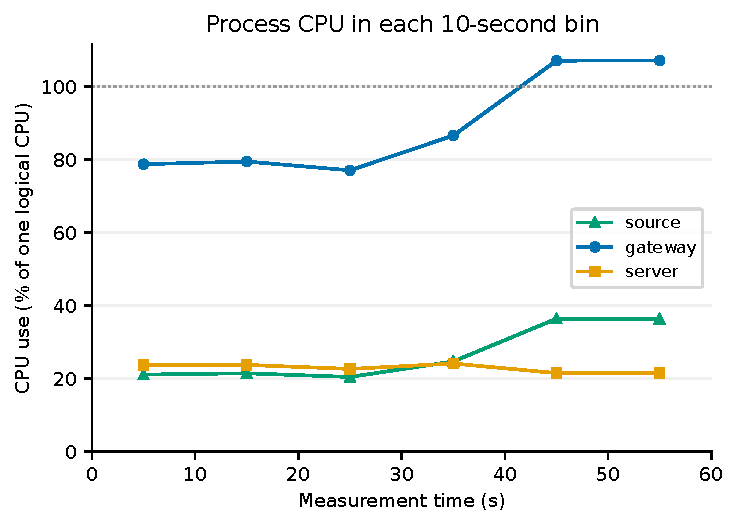
\includegraphics[width=0.88\linewidth]{figures/historical_appendix_within_run_cpu.pdf}
\caption{Historical process CPU in 10 s bins of repeat 1 at nominal 1,024 total messages/s. No repeat error bars are attached to a single-run trace.}
\label{fig:e1r-historical-appendix-within-run-cpu}
\end{figure}


Gateway CPU changed from 78.8\% in the first 10 s bin to 107.2\% in the final bin. This demonstrates changing within-run execution behaviour at a constant configured offered rate; it does not establish a thermal, scheduling or software cause.

\subsection{Queue variation within the same run}

Queue-state intervals were clipped to the same 10 s boundaries and integrated within each bin. The six duration-weighted bin means reproduce the validated whole-window occupancy. The dashed line is the 1,000-message waiting capacity.

\begin{figure}[H]
\centering
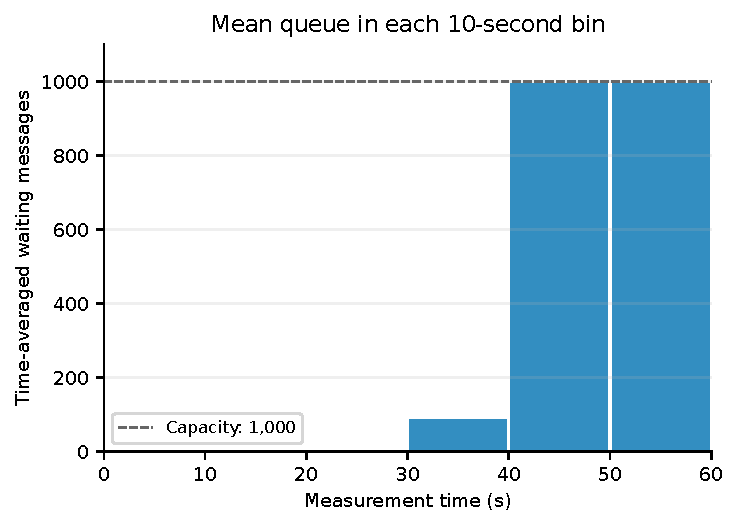
\includegraphics[width=0.88\linewidth]{figures/historical_appendix_within_run_queue.pdf}
\caption{Historical mean FIFO occupancy in 10 s bins of the same repeat-1 run at nominal 1,024 total messages/s.}
\label{fig:e1r-historical-appendix-within-run-queue}
\end{figure}


The first-bin mean queue was 0.95 messages and the final-bin mean was 999.63. Reading this alongside the CPU trace reveals coincident changes in activity and backlog, without identifying a causal explanation.
